\chapter{Analysis} \label{Chapter:Analysis}

\section{Camera frame rate}
\label{ana:cam:fps}

The camera frame rate was calculated as shown by \eref{ana:cam:eq:rate}. The number of lines in a frame can be easily changed by adding dummy lines after the actual frame data. The time required for transmitting synchronisation packet is negligible, thus there are no extra constants in the equation.

\begin{equation}
	f = \frac{\text{Number of lines in a frame data}}{\text{Transmission time of 1 line of data}}
	\label{ana:cam:eq:rate}
\end{equation}

To verify the equation, the transmission times of an entire frame and individual lines were measured using an oscilloscope as shown in \fref{ana:cam:osc:time}. From the cursor measurements shown in the oscilloscope screen captures, the transmission time of an frame is $10.21917 ms$ and $206.45 \mu s$ for 10 lines. It matches the equation precisely. The camera frame rate conversion function in the application was constructed according to these figures.

\begin{figure}[!htb]
  \centering
  \subfigure [Measuring frame interval from synchronisation packets] {
    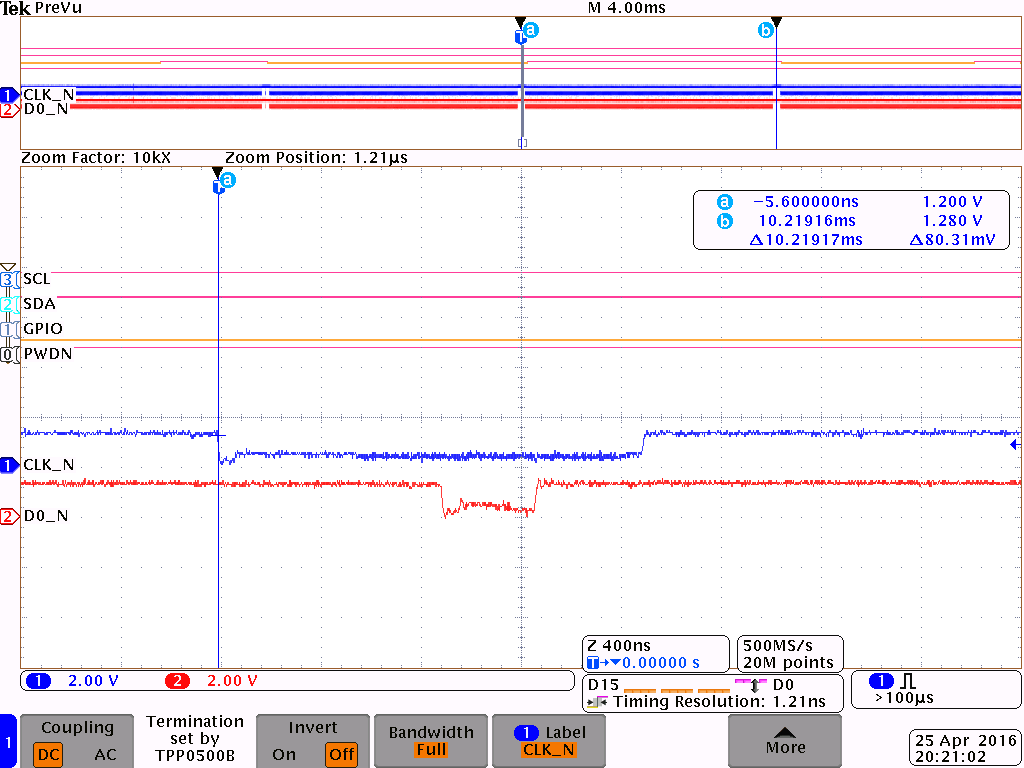
\includegraphics[width=0.9\columnwidth]{camera/osc/frame}
  }
  \subfigure [Measuring transmission time of 10 lines] {
    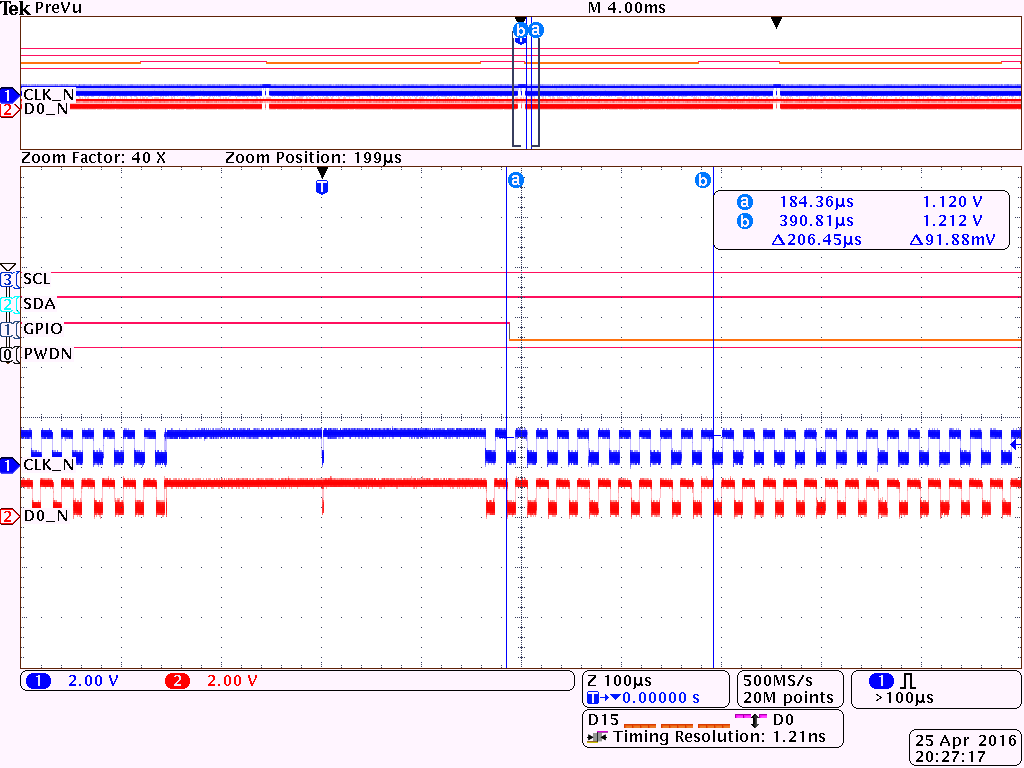
\includegraphics[width=0.9\columnwidth]{camera/osc/line}
  }
  \caption{Measuring the transmission time of an entire frame and individual lines.}
  \label{ana:cam:osc:time}
\end{figure}

However, when experimenting with changing frame rate, a software constraint was discovered. The MIPI-CSI driver developed by NVIDIA can only effectively handle frame rates equal or higher than 5 FPS. For frame rates less than 5 FPS, the camera still functioning as expected, but the driver will be desynchronised. Almost half of frames transmitted from the camera will be lost. As a result, the adaptive operation should not run below 5 FPS.

Another important constraint is the frame rate cannot be changed drastically. When changing the frame interval, camera sensor exposure time, gain control and white balance need to be adjusted at the same time. This is handled by the automatic exposure, gain and white balance adjustment functions on the image sensor processor (ISP) inside camera sensor. The automatic adjustments were implemented with a feedback loop approach. Consequently, when changing the frame interval drastically, the adjustments needed are also significant. As a result, the first few frames captured after such a change will be significantly different from previous frames in brightness and white balance. That is enough to confuse the object tracking algorithms. A software limitation of frame interval changing rate was therefore added in the application. This may be resolved by using software compensation algorithm, but it will required lots of investigations, not possible at this time.

%\todo{BOOM}

\todo{Oscilloscope waveform of frame rate changing.}

\section{\todo{Object tracking algorithms}}

\section{Power consumption modelling}

To measure power consumption, 10 resistors of $10 \Omega$ were connected in parallel to gives a precise $1 \Omega$ resistance and allows high current flow through. Then the resistors was connected in series with the board power supply as shown in \fref{ana:power:sch}. The fan used for CPU cooling can be replaced by passive cooling systems in actual application, thus was powered from an external power source instead of the board during power consumption analysis.

\begin{figure}[H]
  \centering
  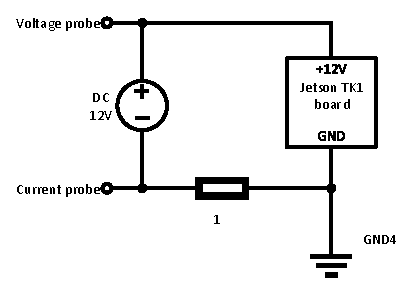
\includegraphics[width=0.6\columnwidth]{ana_power_sch}
  \caption{Schematic of measuring power consumption using oscilloscope.}
  \label{ana:power:sch}
\end{figure}

The average power consumptions of the complete system running the object tracking algorithms at different frame rates were measured as shown in \fref{ana:cam:osc:power}. The current probe was set according to the $1 \Omega$ series resistance, gives accurate current waveform. Maths function on the oscilloscope was used to multiply voltage and current waveforms together, produces power waveform in real-time. The oscilloscope was then set to record 20 million samples of the waveforms in a period of 10 seconds, averaged together to give the average power rating over the period.

\begin{figure}[htb]
  \centering
  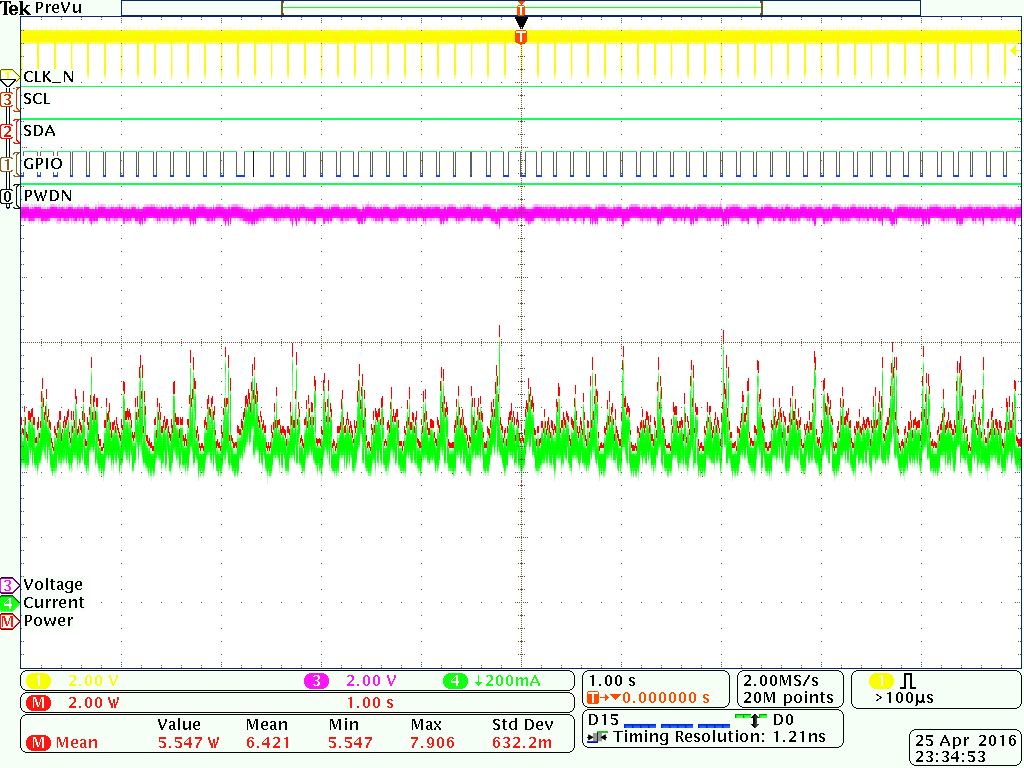
\includegraphics[width=0.9\columnwidth]{camera/osc/power}
  \caption{Screen capture of measuring power consumption using oscilloscope.}
  \label{ana:cam:osc:power}
\end{figure}

Multiple measurements were attempted, then averaged to give the final results shown in \fref{ana:cam:power}. The frame rates chosen were focused on the discrete frame rates used during datasets evaluation.

\begin{figure}[htb]
  \centering
  \subfigure [Detailed data from power consumption measurements] {
    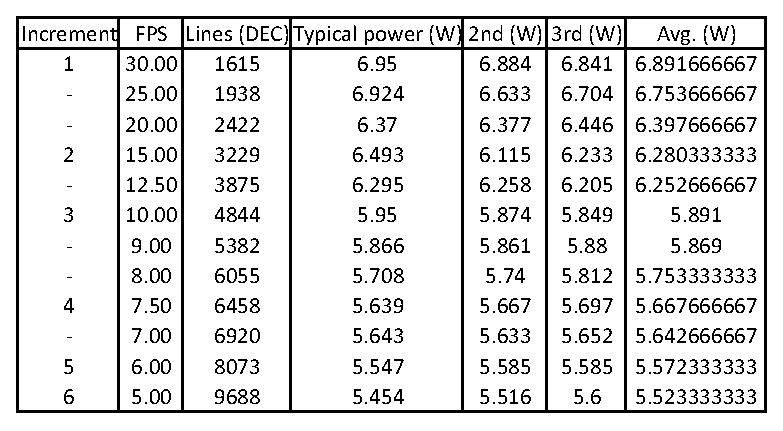
\includegraphics[width=0.55\columnwidth]{ana_cam_data}
  }
  \subfigure [Power consumption ploted against frame rate] {
    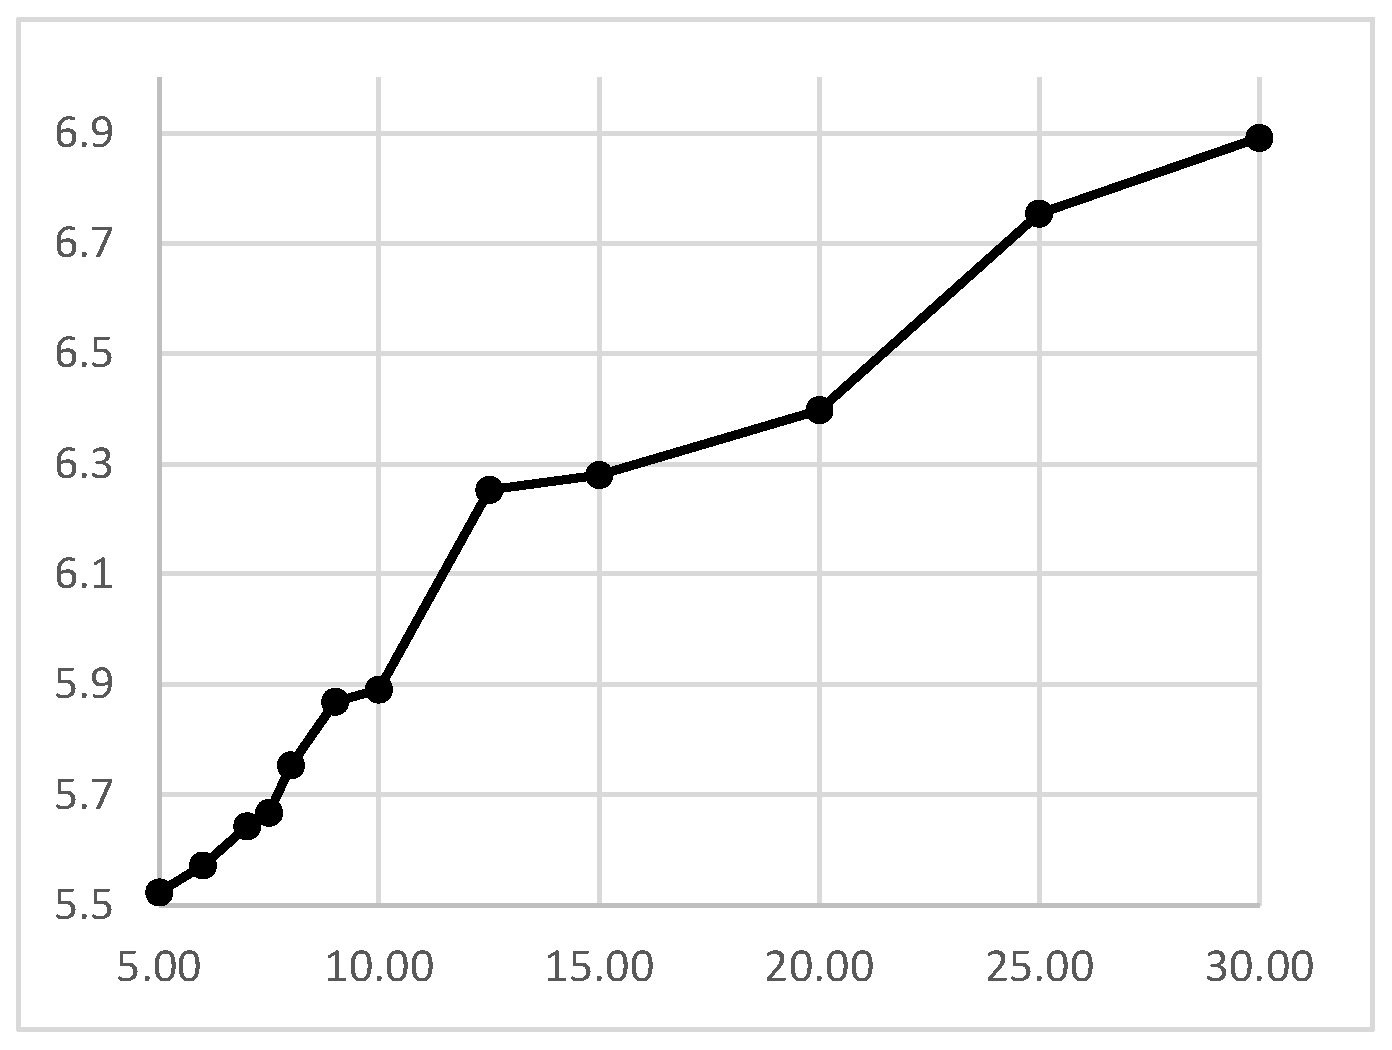
\includegraphics[width=0.35\columnwidth]{ana_cam_chart}
  }
  \centering
  \caption{Power consumptions measured against different frame rates.}
  \label{ana:cam:power}
\end{figure}

%\todo{BOOM}

\section{Power consumption reduction analysis}

Power consumption reduction was analysed using the video datasets from CDNET, to keep input video stream consistent. However, due to the frame images inside the datasets are discrete in time, the frame rate cannot be changed in great precision. The results obtained will only be a rough estimation of the actual performance in actual application.

Some properties of the dataset under test need to be determined first, such as maximum object moving speed and minimum FPS required. This is done by evaluate the dataset without adaptive operation. During the process, the maximum distances objects moved between each frame intervals were recorded. The top $5 \%$ of the distances that are most likely due to errors were removed. \fref{ana:ada} shows the distribution of maximum moving distances after filtering in a dataset. The maximum of those value was considered as the maximum speed an object may travel in the dataset. According to the formulae described in section \ref{imp:ada:metric}, the minimum FPS requirement was then calculated. The optical flow tracking window was set to 32 pixels, as a result most minimum FPS requirements calculated were under 1 FPS. However, to match the constraints of the camera driver as described in section \ref{ana:cam:fps}, the minimum FPS was set to 5 FPS.

\begin{figure}[htb]
  \centering
  \subfigure [Absolute maximum distances objects travelled between frames] {
    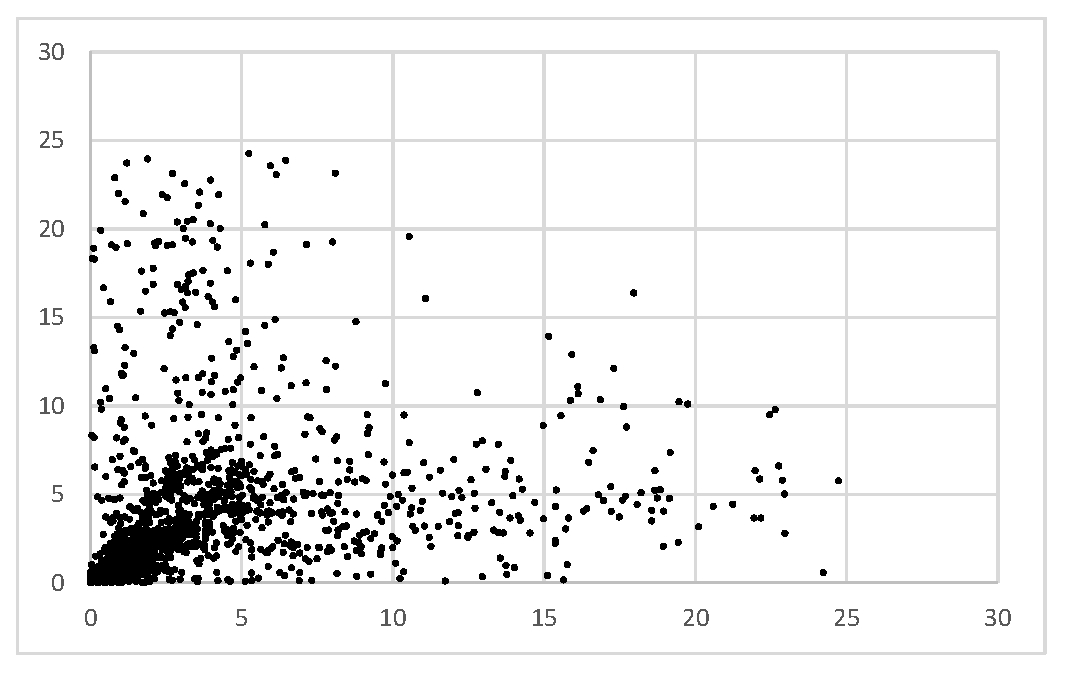
\includegraphics[width=0.45\columnwidth]{ana_ada_xy}
    \label{ana:ada:xy}
  }
  \subfigure [Histogram distribution of maximum distances] {
    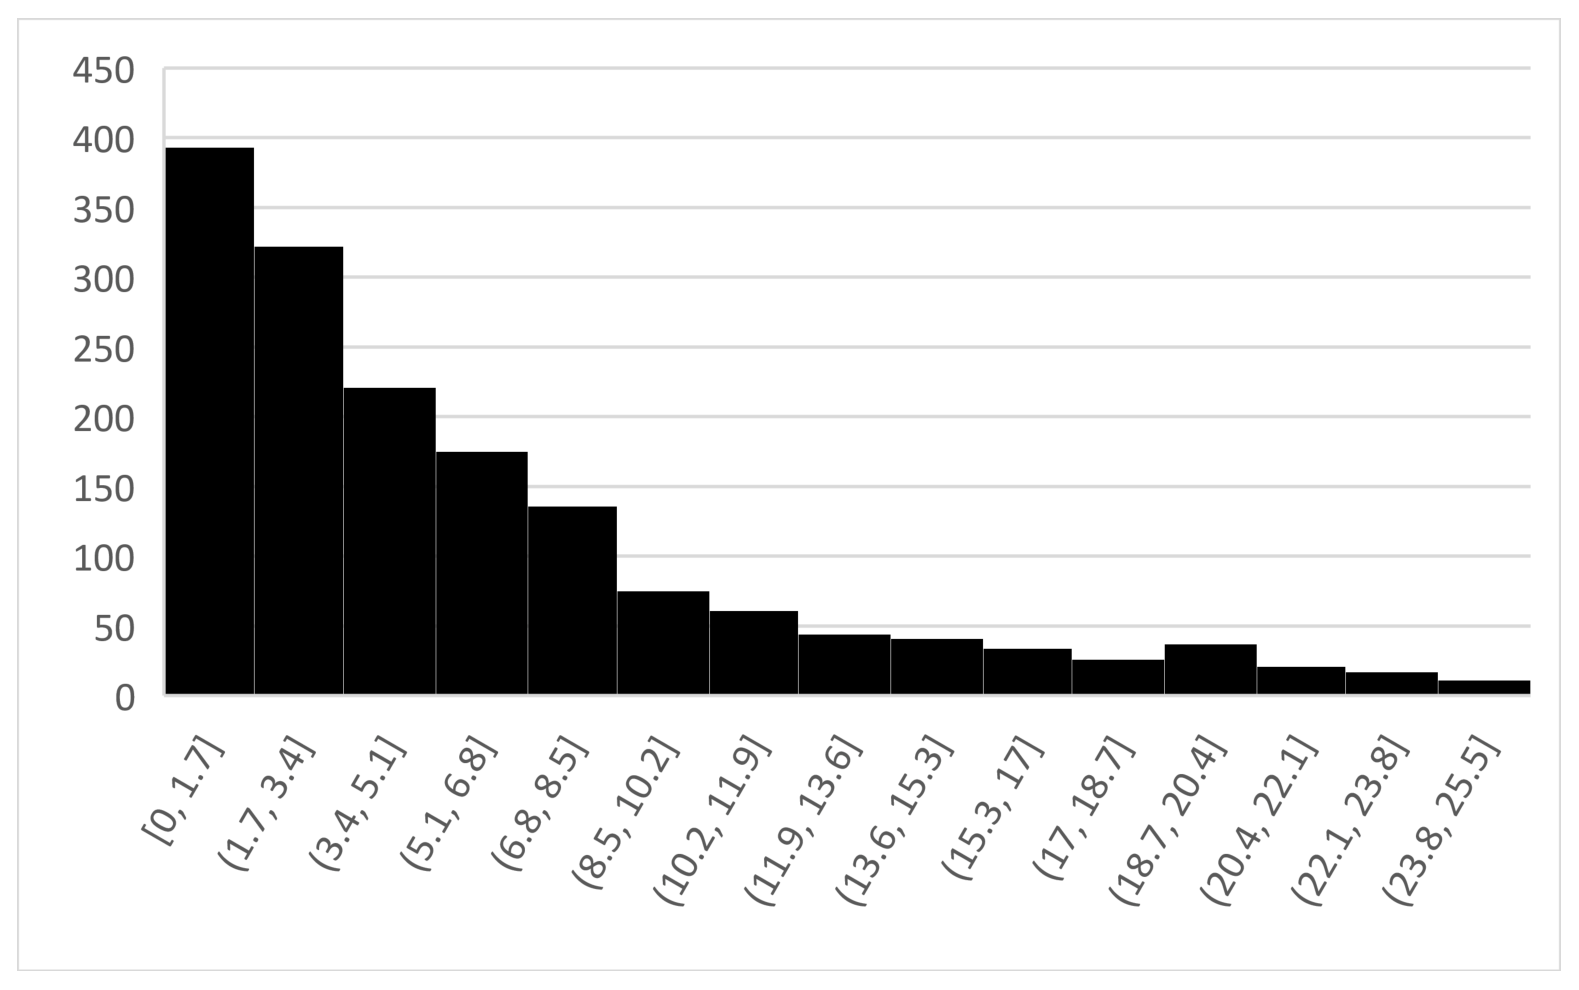
\includegraphics[width=0.45\columnwidth]{ana_ada_histo}
    \label{ana:ada:histo}
  }
  \caption{Filtered distributions from CDNET highway dataset.}
  \label{ana:ada}
\end{figure}

Moving blobs that are continuously connected by the tracking algorithm across frames were considered as being tracked. The speed of objects moving in the datasets are relatively low to the frame rate, all objects in the datasets evaluated are considered as being tracked regardless of adaptive operation.

By applying the power consumption model, the power consumption reduction can be estimated, summarised in \fref{ana:summary}.

\begin{figure}[htb]
  \centering
  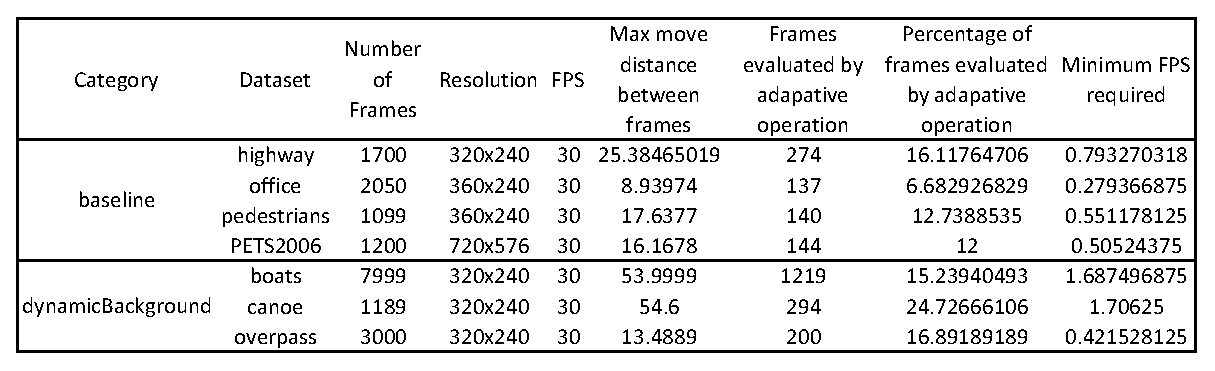
\includegraphics[width=\columnwidth]{ana_summary}
  \caption{Summary of results from evaluated CDNET datasets.}
  \label{ana:summary}
\end{figure}
